% !TEX encoding = UTF-8 Unicode

\documentclass[a4paper]{article}

\usepackage{color}
\usepackage{url}
\usepackage[T2A]{fontenc} % enable Cyrillic fonts
\usepackage[utf8]{inputenc} % make weird characters work
\usepackage{graphicx}

\usepackage[english,serbian]{babel}

\usepackage[unicode]{hyperref}
\hypersetup{colorlinks,citecolor=green,filecolor=green,linkcolor=blue,urlcolor=blue}

\newtheorem{primer}{Primer}[section]

\DeclareUnicodeCharacter{0301}{\'{c}}

\title{Roboti kao nastavnici\small \\Seminarski rad u okviru kursa\\Tehničko i naučno pisanje\\Matematički fakultet}
\author{Jovan Mijajlović, jovan.mijajlovic03@gmail.com\\Miona Sretenović, sretenovicmiona7@gmail.com\\Mina Protić, minaproticc@gmail.com\\Mihailo Marković, mihailoo003@gmail.com}
\date{11.~novembar 2022}

\begin{document}
\maketitle
\tableofcontents
\newpage

\section{Uvod}

Roboti stižu u školske klupe!
Roboti, kao pomoć nastavnicima informatike, stižu u školske klupe. Đaci će se po prvi put uveriti da programiranje nije apstraktno, jer će ono što su isprogramirali izvršavati roboti. Dosad se za tu obuku prijavilo više od 400 nastavnika, a plan je da svi nastavnici informatike budu uključeni, ali i da svaka škola dobije po pet robota. Međutim, postavlja se pitanje koliko je to izvodljivo?
Da bismo govorili o ovoj temi moramo se prvo upoznati sa time šta su roboti a šta nastavnici.

\section{Šta su roboti?}
Robot jeste elektro-mehanička jedinica koja je u stanju da autonomno, po nekom programu, ili pod kontrolom čoveka izvodi određene zadatke. Roboti se koriste za izvođenje zadataka opasnih, teških ili napornih za ljude. Na primer sakupljanje nuklearnog otpada ili slaganje velikog broja žica prema boji, kao i repetitivne poslove gde se zahteva istrajnost i preciznost, kao što je sklapanje motora i šasije automobile.
Roboti koji imaju oblik ljudskog tela se još zovu humanoidni roboti. Ako je uz ovo još i svrha da se po njihovim ostalim karakteristikama, kao što su kretanje, govor, gestikulacije itd, što više približe ljudskim bićima, radi se o androidima. Ovaj termin se ipak češće sreće u naučnoj fantastici.
Inteligenciju koju robot poseduje čini u stvari program ili sistem programa, koji određuje sposobnost robota da prepozna određene situacije i da se u njima snađe ili ih rešava, ponašajući se na pravi način ili čak iz sopstvenog iskustva uči kako da se snalazi u novim situacijama i rešava nove probleme. Ova vrsta inteligencije se zove još i veštačka inteligencija i predstavlja zasebnu granu nauke. Izraz „robot“ se prvi put pominje u drami čehoslovačkoga pisca Karela Čapeka „R. U. R.“. Za termin robot zaslužan je njegov brat Josef Čapek. Reč je nastala na čehoslovačkom jeziku pa se onda proširila na ceo svet.
Roboti mogu da budu autonomni ili poluautonomni i u opsegu su od humanoidnih kao što je Hondin Napredni korak u inovativnoj mobilnosti (ASIMO) i TOSY-jev TOSY robot koji igra ping pong (TOPIO) do industrijskih robota, medicinskih operativnih robota, onih koji pomažu pacijentima, robota za pseću terapiju, kolektivno programiranih rojskih robota, bespilotnih letelica kao što je MQ-1 predator, i mikroskopskih nano robota. Putem oponašanja izgleda živih bića ili automacije pokreta, robot može da pruži osećaj inteligencije ili sopstvenog razmišljanja. Očekuje se da će doći do proliferacije autonomnih predmeta u narednim dekadama, pri čemu su kućna robotika i autonomna kola među vodećim oblastima primene.


\begin{figure}[h!]
\begin{center}
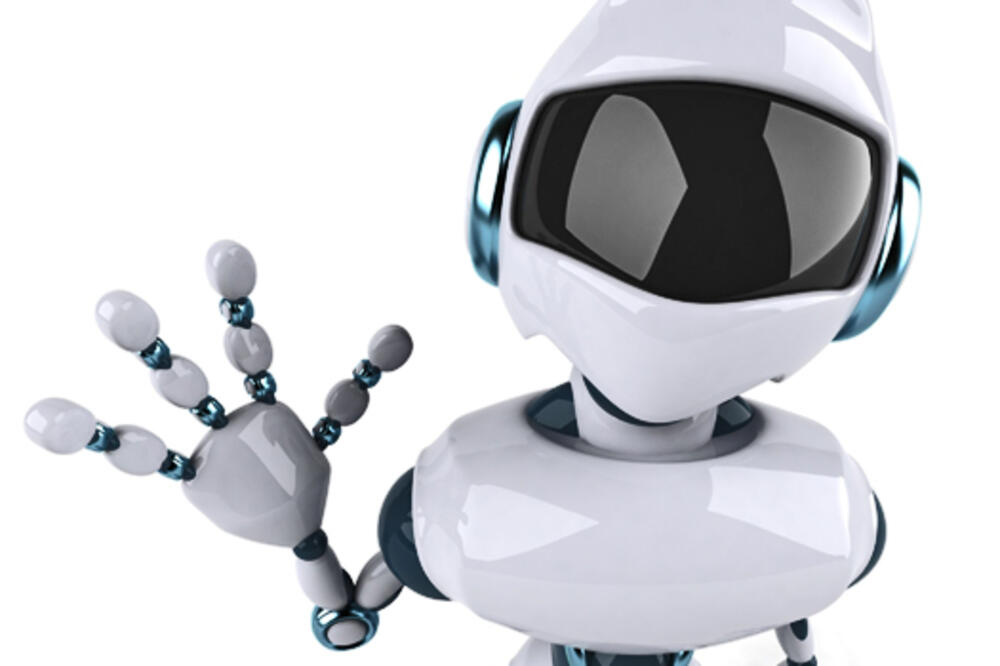
\includegraphics[scale=0.3]{robotm.jpg}
\caption{Robot}
\end{center}
\label{fig:robot}
\end{figure}

\newpage
\section{Šta su nastavnici?}
Nastavnik je stručna osoba visokih radnih, obrazovnih i etičkih kvaliteta edukovana za rad u vrtiću, školi ili fakultetu za određen predmet. On mora da zadovolji niz specifičnih zahteva kao što su: svesna motiviranost za zvanje, potpuniji sastav opšteg i stručnog obrazovanja, visoke intelektualne sposobnosti, crte ličnosti adekvatne sastavu vrednosti u društvu, visoki nivo zrelosti ličnosti, kao i visoki nivo lične kulture.

\begin{figure}[h!]
\begin{center}
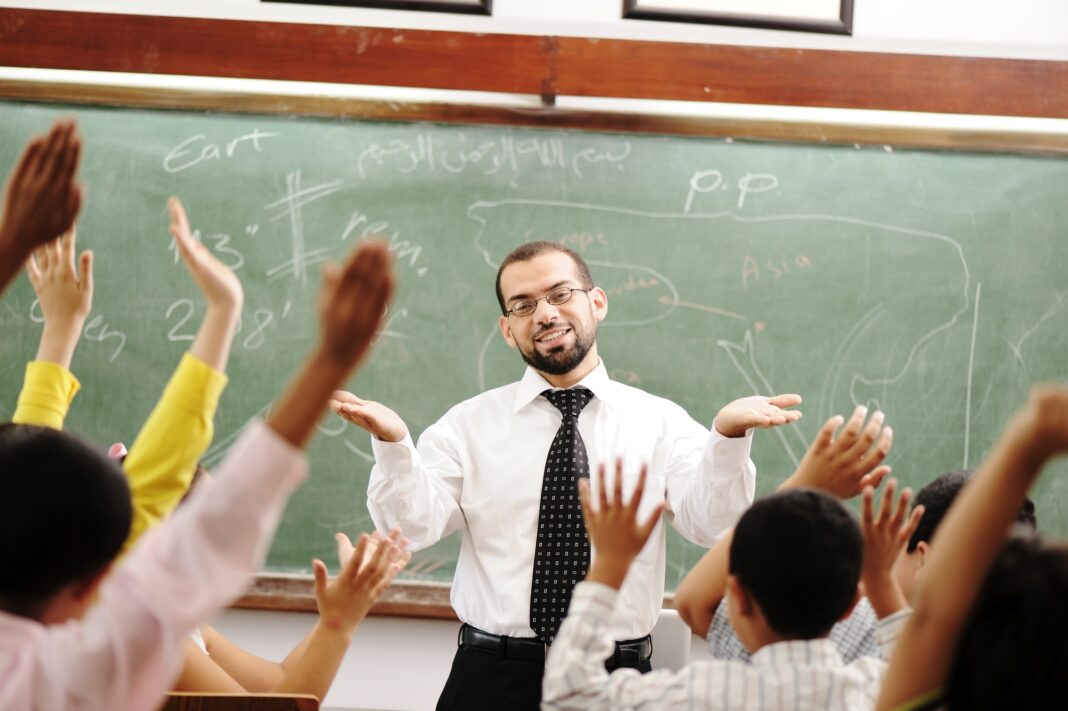
\includegraphics[scale=1.2]{nastavnik.jpg}
\caption{Nastavnik}
\end{center}
\label{fig:nastavnik}
\end{figure}

\newpage
\subsection{Entuzijazam nastavnika}
Utvrđeno je da nastavnici koji su pokazali entuzijazam prema materijalima kursa i studentima mogu stvoriti pozitivno iskustvo učenja. Ovi nastavnici ne predaju napamet, već pokušavaju da osnaže svoje predavanje materijima kursa svakog dana. Nastavnicima koji ponavljaju isti nastavni plan i program može biti izazov da održe svoj entuzijazam, kako se njihova dosada sa sadržajem ne bi negativno odražavala na njihove učenike. Nastavnike entuzijaste njihovi učenici ocenjuju više od nastavnika koji nisu pokazali mnogo entuzijazma za materijale kursa.
Nastavnici koji pokazuju entuzijazam imaju veću verovatnoću da imaju angažovane, zainteresovane i energične učenike koji su radoznali da nauče predmet. Nedavno istraživanje je otkrilo korelaciju između entuzijazma nastavnika i unutrašnje motivacije učenika da uče i vitalnosti u učionici. Kontrolisane, eksperimentalne studije koje istražuju intrinzičnu motivaciju studenata pokazale su da neverbalni izrazi entuzijazma, kao što su demonstrativna gestikulacija, dramatični pokreti koji su različiti i emocionalni izrazi lica, dovode do toga da studenti prijavljuju više nivoe unutrašnje motivacije za učenje. Ali čak i ako se pokazalo da entuzijazam nastavnika poboljšava motivaciju i povećava angažovanje u zadatku, to ne mora nužno da poboljša ishode učenja ili pamćenje materijala.
Postoje različiti mehanizmi pomoću kojih entuzijazam nastavnika može olakšati viši nivo unutrašnje motivacije. Entuzijazam nastavnika može doprineti atmosferi energije i entuzijazma u učionici koja podstiče interesovanje i uzbuđenje učenika u učenju predmeta. Nastavnici entuzijasti mogu takođe dovesti do toga da učenici postanu samoopredeljeni u sopstvenom procesu učenja. Koncept pukog izlaganja ukazuje na to da nastavnikov entuzijazam može doprineti očekivanjima učenika o intrinzičnoj motivaciji u kontekstu učenja. Takođe, entuzijazam može delovati kao „motivaciono ulepšavanje“, povećavajući interesovanje učenika raznovrsnošću, novinom i iznenađenjem entuzijastičnog nastavnika koji predstavlja materijal. Konačno, može se primeniti i koncept emocionalne zaraze: učenici mogu postati suštinski motivisani uhvaćenim entuzijazmom i energijom nastavnika.

\end{document}
